\documentclass[twocolumn,superscriptaddress,10pt,showpacs,prl]{revtex4}%
\renewcommand\baselinestretch{1}
%\usepackage{mathbbold}
\usepackage{mathrsfs}%

\textheight 260mm

\oddsidemargin=0mm

\topmargin=40pt
\renewcommand
\baselinestretch{1}
\voffset   -2.75cm
\hoffset  -1.25cm
\usepackage{natbib}
\usepackage{bm}
\usepackage{amsmath}
\usepackage{threeparttable}
\usepackage{amssymb}

\usepackage{amsfonts}

\usepackage[colorlinks,CJKbookmarks,linkcolor=blue]{hyperref}
\usepackage{color}
\usepackage{booktabs}  %���岻ͬ��ϸ�ķָ���
\usepackage{tabularx}  %������
\usepackage{graphicx}%
\renewcommand{\arraystretch}{1.5}
\renewcommand{\textfraction}{0.15}
\renewcommand{\topfraction}{0.85}
\renewcommand{\bottomfraction}{0.65}
\renewcommand{\floatpagefraction}{0.60}
\begin{document}
\title{Experimentally simulating the violation of Bell-type inequalities for three qubits by NMR}
\author{Changliang Ren}
\email{clren@mail.ustc.edu.cn} \affiliation{Department of Modern
Physics, University of Science and Technology of China, Hefei,
Anhui, 230026, China}
\author{Dawei Lu}
\email{sioldw@mail.ustc.edu.cn} \affiliation{Hefei National
Laboratory for Physical Sciences at Microscale, Hefei, Anhui,
230026, China}
\author{Mingjun Shi}
 \affiliation{Department of Modern Physics, University of
Science and Technology of China, Hefei, Anhui, 230026, China}
\author{Jiangfeng Du}
 \affiliation{Department of Modern Physics, University of
Science and Technology of China, Hefei, Anhui, 230026, China}
\affiliation{Hefei National Laboratory for Physical Sciences at
Microscale, Hefei, Anhui, 230026, China}
\begin{abstract}
We simulate the violation of MABK inequality for a three-qubit GHZ
state in a NMR system. Furthermore, for generalized GHZ states, we test two different Bell's inequalities, i.e., MABK inequality and Chen's
inequality. The experimental results show
that Chen's inequality is more efficient than MABK inequality for any generalized GHZ entangled states.
\end{abstract}

\pacs{03.65.Ud, 76.60.-k}\maketitle
\subsection*{I. Introduction}
\begin{frame}
 In 1964, Bell showed that in all local realistic
theories, correlations between the outcomes of measurements in
different parts of a physical system satisfy a certain class of
inequalities \cite{Bell}. However, it was easy to find that entangled
states violate these inequalities in quantum mechanics, which shows the crucial conflict between classical theory and
quantum mechanics. Hence, Bell's work was described as "the
most profound discovery of science" \cite{Stapp} or "one of the
greatest discoveries of modern science" \cite{Zukowski}. Later, many
important generalizations, including the Clauser-Horne-Shimony-Holt
(CHSH) \cite{CHSH} and Mermin-Ardehali-Belinskii-Klyshko (MABK)
inequalities \cite{MABK} have been developed. More recently, Werner
and Wolf and \.{Z}ukowski and Brukner (WWZB) derived a set of
multipartite Bell inequalities, by using two dichotomic observables
per site \cite{WWZB}. There has been increasing interest
in the subject of Bell's inequalities, because of not only fundamental
problems of quantum mechanics, but also their relation to
quantum communication \cite{ Brukner, Brassard, Scarani} and quantum
cryptography \cite{Chen,Acin and Gisin}. For example, the security
of some quantum communication protocols are based on the
loophole-free violation of Bell inequalities \cite{Acin and Gisin,
Barrett, Acin and Brunner}. Furthermore, Bell��s inequalities can be
a useful tool to detect entanglement which is a powerful
computational resource in quantum computation \cite{Nielsen}.

Various experiments to test Bell inequality have been performed in
a wide range of systems including photons \cite{Freedman, Aspect,
Weihs}, atoms systems \cite{Moehring, Matsukevich1, Matsukevich2},
atomic ensembles \cite{Matsukevich3, Chou}, and trapped ions
\cite{Rowe}. Recently, an experiment to simulate the violation of
CHSH inequality has been carried out in an NMR system \cite{Souza}. These experiments were mainly
carried out on the maximal entangled states, such as Bell states and
standard GHZ states, etc, rarely on nonmaximal entangled states, such
as generalized GHZ states. However, many phenomena can be disclosed by nonmaximal entangled states,
for instance, the nonmaximal entangled states make the maximal violation of many Bell-type
inequalities \cite{Acin and Durt,
Methot and Scarani}. There are still many open problems about the Bell-type inequalities with
nonmaximal entangled states. Therefore, it is
interesting and meaningful to study the case of  nonmaximal entangled states.

For three-qubit generalized GHZ states
\begin{equation}\label{generalized GHZ state} \left\vert
\Psi \right\rangle=\cos\theta\left\vert 000 \right\rangle+\sin
\theta\left\vert 111 \right\rangle,
\end{equation}
which $\theta\in[0, \frac{\pi}{2}]$,
 Scarani and Gisin
\cite{Scarani and Gisin} firstly found that there exist a region of
them satisfying the MABK inequality. It is shown that for $\theta\leq
\pi/12$ or $\theta\geq5\pi/12$ the states \eqref{generalized GHZ
state} do not violate the three-qubit MABK inequality. Later on,
\.{Z}ukowski \emph{et.al} proved that \cite{Zukowski and
Brukner and Laskowski and Wiesniak} ($i$) for $N=even$, the
generalized GHZ states violates the WWZB inequality, rather than MABK inequalities;
($ii$) for $N=odd$ and
$sin(2\theta)\leq1/\sqrt{2^{N-1}}$, ( the correlations between
measurements on qubits in the generalized GHZ state satisfy all Bell
inequalities for correlation functions, which involve two dichotomic
observables per local measurement station ??? ). Chen and Wu \emph{et al.} developed several Bell
inequalities in terms of both probabilities and correlation
functions for three qubits, which can be numerically
violated by any pure entangled state \cite{J. L. Chen, C. F. Wu}.
Recently, a more significant progress was achieved by K. Chen \emph{et
al.} \cite{k.Chen}. They presented a family of Bell inequalities
involving only two measurement settings of each observer for $N>2$
qubits, which is violated by any $N$-qubit generalized GHZ
state, and moreover the amount of maximal violation
grows exponentially as $2^{(N-2)/2}$.

There are much work on the theoretical aspect, whereas no experiments aim to display so far.
In this paper, we simulate the violation of two different Bell-type inequalities, i.e., MABK inequality \cite{MABK} and Chen's inequality \cite{k.Chen},
for a three-qubit GHZ state as well as for generalized GHZ states in an NMR system. The experimental
results clearly shows that the high efficiency of Chen's inequality and the limitation of MABK inequalityfor any generalized GHZ entangled states . Our experimental results are well coincident with the
prediction of quantum mechanics.

\end{frame}
\subsection*{II.Simulation violation of MABK inequality for GHZ state}
\begin{frame}
Let us consider such a scenario: there are three observers Alice
(\emph{A}), Bob (\emph{B}), and Charlie (\emph{C}), each having one
qubit. The formulation of the MABK inequality is based on the
assumption that every observer is allowed to choose one observable between two
dichotomic observables. Denote the outcome of observer $X$'s
measurement by $X_{i}, X=A,B,C$, with $i=1,2$. Under the assumption
of local realism, each outcome can either take value $+1$ or $-1$.
In a specific run of the experiment, the correlations between the
measurement outcomes of all three observers can be represented by
the product $A_{i}B_{j}C_{k}$, where $i , j , k=1, 2$. In a local
realistic theory, the correlation function of the measurements
performed by all three observers is the average of $A_{i}B_{j}C_{k}$
over many runs of the experiment,  The MABK inequality reads as
\cite{MABK}
%\begin{widetext}%
\begin{eqnarray}\label{MABK}
&|&E(A_{1},B_{2},C_{2})+E(A_{2},B_{1},C_{2})+\nonumber\\
&&E(A_{2},B_{2},C_{1})-E(A_{1},B_{1},C_{1}){}|\leq2.
\end{eqnarray}
%\end{widetext}%
We denote the left-hand side of the MABK inequality by
$|\mathcal{B}_{MABK}|$ where $-2\leq\mathcal{B}_{MABK}\leq2$. In any
local hidden variable (LHV) theory, the absolute value of a
particular combination of correlations is bounded by 2. However, if
one turns to quantum mechanics, this inequality can be violated. For
MABK inequality, the maximal violation allowed by quantum mechanics
is $4$ \cite{Scarani and Gisin}, which for standard GHZ state,
\begin{equation}\label{standard GHZ state}
\left\vert \Phi \right\rangle=\frac{1}{\sqrt{2}}(\left\vert 000
\right\rangle+\left\vert 111 \right\rangle).
\end{equation}

To prepare standard GHZ state from $\left\vert 000 \right\rangle$,
we used the network as shown in Fig.1, by selecting the rotation
angle $2\theta=\pi/2$. After that, we will measure the spin
projection $\bm{\sigma\cdot n}$, where
$\bm{\sigma}=(\sigma_x,\sigma_y,\sigma_z)$ is the vector form of
Pauli matrices and the two measurement directions for every qubit we
chose here are $\bm{n_1}=(1,0,0)$ and
$\bm{n_2}=(\cos\alpha,\sin\alpha,0)$.

For this special spin projection measurement, the theoretical result
of $\mathcal{B}_{MABK}$ is (for convenience we just ignore the
absolute value sign)
\begin{equation}
\mathcal{B}_{MABK}=3( \cos^{2}\alpha-\sin^{2} \alpha)-1,
\end{equation}
demonstrating that for $\alpha=0.3041\pi\sim0.6959\pi$ the result
violates MABK inequality and reach the maximal violation value $4$
when $\alpha=\pi/2$, as shown in Fig.4.
\begin{figure}[h] \centering
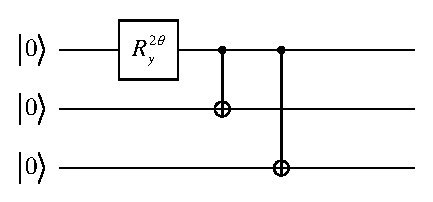
\includegraphics[width=0.6\columnwidth]{net.eps}
\caption{\footnotesize{Quantum network for creating a generalize
GHZ state. The initial state is $\left\vert 000 \right\rangle$.
After rotating qubit 1 by the angle $2\theta$ about Y axis, we get
$\cos\theta\left\vert 000 \right\rangle+\sin\theta\left\vert 100
\right\rangle$.Then through two control gates CNOT$_{12}$ and
CNOT$_{13}$, a generalize GHZ state $\cos\theta\left\vert 000
\right\rangle+\sin\theta\left\vert 111 \right\rangle$ will be
created.}}
\end{figure}

For NMR experimental implementation, there are still two problems to
be solved. Firstly, the thermal equilibrium state of a NMR system at
room temperature is highly mixed. We can use pseudo-pure state(PPS)
\cite{Gershenfeld} technique to overcome this, that the initial
state is transformed to
\begin{equation}
\rho_{pps}=\frac{(1-\varepsilon)}{2^n}I_{2^n}+\varepsilon\left\vert
\varphi\right\rangle\left\langle\varphi\right\vert,
\end{equation}
which is a mixture of the totally mixed state $I_{2^n}$ unchanged
when applying with unitary transformations and a pure state
$\left\vert \varphi\right\rangle$ which we set to be $\left\vert 0
\right\rangle$ in our experiment with the polarization
$\varepsilon=10^{-5}\sim10^{-6}$. So ignoring $I_{2^n}$ which does
not affect NMR experiments and using the entanglement(strictly,
pseudo-entanglement) of the pure part, we can simulate violation of
the Bell-type inequalities we mentioned in this letter. Another
problem is only the spin projection values under computational basis
can be directly measured. The solution is to rotate the state or
density matrix instead of changing the projective direction,
\begin{eqnarray}
M=Tr(\rho\cdot M_{1})=Tr(\rho\cdot U^{+}M_2U) \nonumber\\
=Tr(U\rho U^{+}\cdot M_2),
\end{eqnarray}
where $M_1$ and $M_2$ are the desired and experimental
measurements, respectively. $U$ is one unitary operation satisfying
$M_1=U^{+}M_2U$. In NMR experiments we can apply $U$ to the density
matrix and then perform measurement of $M_2$, which is equivalent to
measuring $M_1$.
\begin{figure}[h] \centering
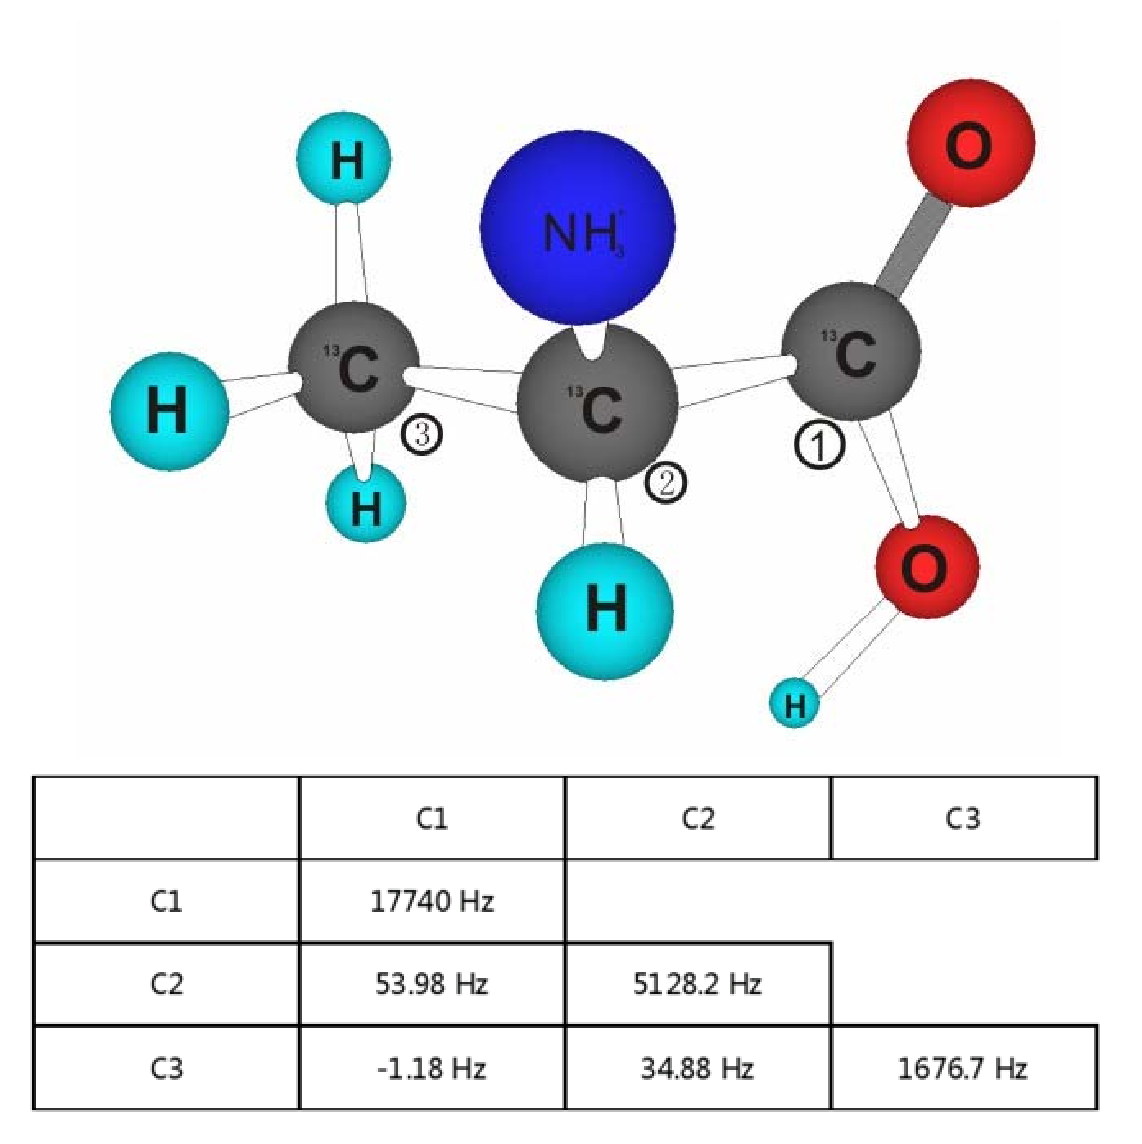
\includegraphics[width=0.7\columnwidth]{structure.eps}
\caption{\footnotesize{Molecular structure and Hamiltonian
parameters for alanine. The diagonal elements are the chemical
shifts of the three carbon nuclei and the off-diagonal elements are
the J-coupling strengths. }}
\end{figure}

All experiments were performed at room temperature on a Bruker
Avance 400MHz NMR spectrometer. We used the spins of three
${}^{13}\!C$ nucle in alanine dissolved in $D_2 O$. The system
Hamiltonian can be written as
\begin{equation}
H_{sys}=\sum_{i=1}^3 \omega_i I_z^i+2\pi\sum_{i<j}^3 J_{ij} I_z^i
I_z^j,
\end{equation}
with the Larmor angular frequencies $\omega_i$ in the rotating frame
and $J$-coupling constants $J_{ij}$, whose values are listed in
Fig.2.

The whole experiment was divided into three steps. Firstly, to
prepare $\rho_{pps}$ from the thermal equilibrium state by using the
spatial average technique \cite{Cory}. Secondly, to prepare a
standard GHZ state by using the network in Fig. 1 with $2\theta=\pi/2$. Finally, to rotate the
required qubits and execute the projective measurements.

In order to improve the accuracy of radio frequency (RF) pulses, we
used strongly modulating pulse (SMP) techniques \cite{Fortunato}. We
also maximized the effective gate fidelity by averaging over a
weighted distribution of RF field strengths to overcome the
inhomogeneity of the RF fields over the sample. The gate fidelity we
calculated for every pulse is higher than 0.995 considering the RF
field inhomogeneity. The range of the pulse lengths are about from
$200\sim 700\mu s$.
\begin{figure}[h] \centering
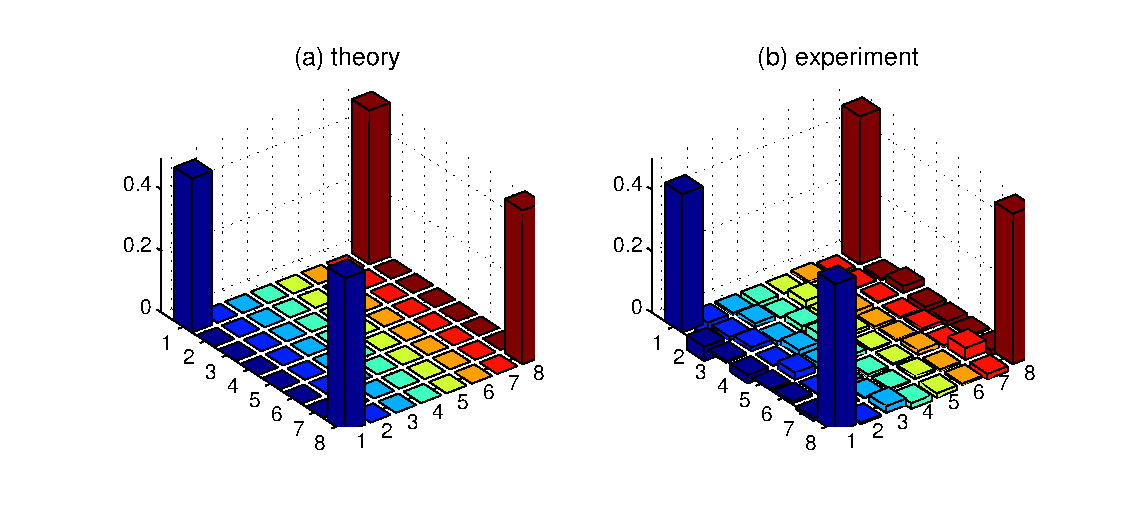
\includegraphics[width=1\columnwidth]{tomo.eps}
\caption{\footnotesize{Theoretical (a) and experimental (b) density
matrices of the standard GHZ state $(\left\vert 000
\right\rangle+\left\vert 111 \right\rangle)/{\sqrt{2}}$. }}
\end{figure}

Fig.3 (b) shows a full state tomography of the standard GHZ state prepared in
experiment. The overall fidelity is
\begin{equation}
F=\frac{Tr(\rho_{th}\rho_{exp})}{\sqrt{(Tr(\rho^2_{th})Tr(\rho^2_{exp}))}}=0.98,
\end{equation}
We took several sets of observers to do the corresponding
measurement on standard GHZ state. The experimental result is shown in the Fig.4,
where the blue squares stand for the experiment results, and the red
thick line stands for the theoretical result. Clearly, the
experiment results are in excellent agreement with the theoretical
expectation of quantum mechanics.
\begin{figure}[h] \centering
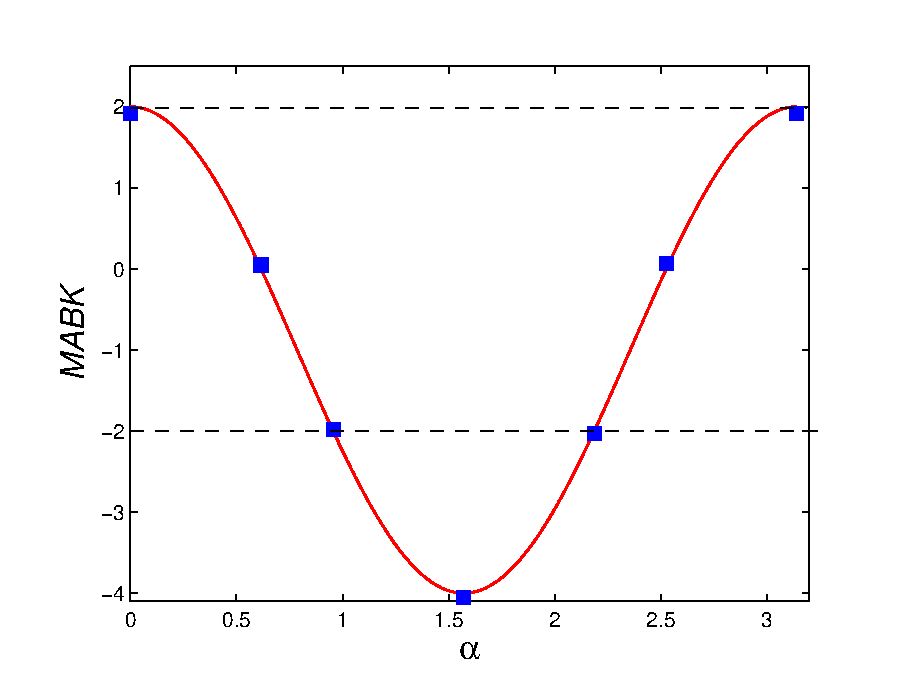
\includegraphics[width=0.7\columnwidth]{MABK1.eps}
\caption{\footnotesize{ $\mathcal{B}_{MABK}$ as a function of
$\alpha$. The red thick line stands for the theoretical expectation,
and the blue square stands for the experimental data.}}
\end{figure}



\end{frame}
\subsection*{III. Simulation violation of MABK inequality for generalize GHZ states}
\begin{frame}
So far, almost all previous Bell experiments were performed on
maximal entangled states, such as Bell states and standard GHZ states.
Recently, sorts of unexpected properties about nonmaximal entangled
states have been shown\cite{Acin and Durt, Methot and Scarani}.
Therefore, we will next simulate the violation of MABK inequality for
generalized GHZ states.

In this experiment, we choose the directions of the two measurements
for every particles are $\bm{n_1}=(1,0,0)$ and $\bm{n_2}=(0,1,0)$.
For these special spin projection measurements, the theoretical
result of $\mathcal{B}_{MABK}$ for generalized GHZ states satisfies
such a function,
\begin{equation}\label {1}
|\mathcal{B}_{MABK}|=|-4\sin(2\theta)|.
\end{equation}
From \eqref{1}, one can see that the maximal violation is obtained
when $\theta=\frac{\pi}{4}$ just the standard GHZ state. Obviously,
the MABK inequality is efficient only in the region of $\theta\in[\frac{\pi}{12},
\frac{5\pi}{12}]$; in other words, only in such region
the inequality can be violated.

We measured a set of generalized GHZ states with particular angle
$\theta$.
 The result is shown in Fig.5 which shows a good  consistence with the prediction of quantum theory.
\begin{figure}[h]
\begin{center}
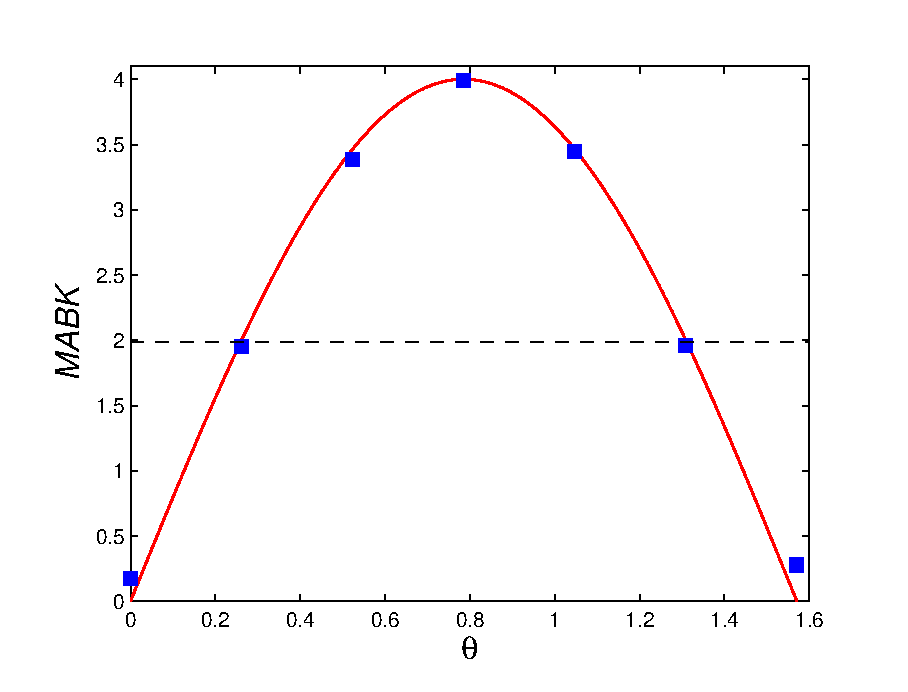
\includegraphics[width=0.35\textwidth]{MABK2.eps}
\caption{\footnotesize{The values of $\mathcal{B}_{MABK}$ as a
function of $\theta$. The red thick line stands for the theoretical
expectation, and the blue squares stand for the experiment data.}}
\end{center}
\end{figure}
\end{frame}
\subsection*{IV. Simulation violation of Chen's inequality for generalize GHZ states}
\begin{frame}
For a three-qubit system, Chen's inequality can be written as
\begin{widetext}%
\begin{eqnarray}
\mathcal{B}_{Chen}=\frac{1}{2}(E(A_{1},B_{1},C_{1})+E(A_{1},B_{2},C_{1})+E(A_{2},B_{1},C_{1})-
E(A_{2},B_{2},C_{1})+E(A_{1},B_{1},C_{2})+\nonumber\\
E(A_{1},B_{2},C_{2})+
E(A_{2},B_{1},C_{2})-E(A_{2},B_{2},C_{2}))+E(C_{1})-E(C_{2}),
\end{eqnarray}
\end{widetext}%
 $|\mathcal{B}_{Chen}|\leq2$ in the LHV model.

In experiment, based on [29], we take the directions of two
measurement about $A$ and $B$ as $\bm{n_1}=(1,0,0)$ and
$\bm{n_2}=(0,1,0)$. For $C$, the directions of two measurement are
$\bm{n_1}=(\sin\alpha\cos(-\frac{\pi}{4}),\sin\alpha\sin(-\frac{\pi}{4}),\cos\alpha)$
and
$\bm{n_2}=(\sin(\pi-\alpha)\cos(-\frac{\pi}{4}),\sin(\pi-\alpha)\sin(-\frac{\pi}{4}),\cos(\pi-\alpha))$,
where
\begin{eqnarray}
\alpha=\tan^{-1}[\sqrt{2}\tan(2\theta)],\quad\quad\quad\quad
   0\leq\theta\leq\frac{\pi}{4}\nonumber
\\\alpha=\tan^{-1}[\sqrt{2}\tan(2\theta)]+\pi,\quad\quad
   \frac{\pi}{4}\leq\theta\leq\frac{\pi}{2}
\end{eqnarray}
Then, we obtain $\mathcal{B}_{Chen}$ as
\begin{equation}
\mathcal{B}_{Chen}=2[2\sin^{2}(2\theta)+\cos^{2}(2\theta)]^{1/2}.
\end{equation}
\begin{figure} \centering
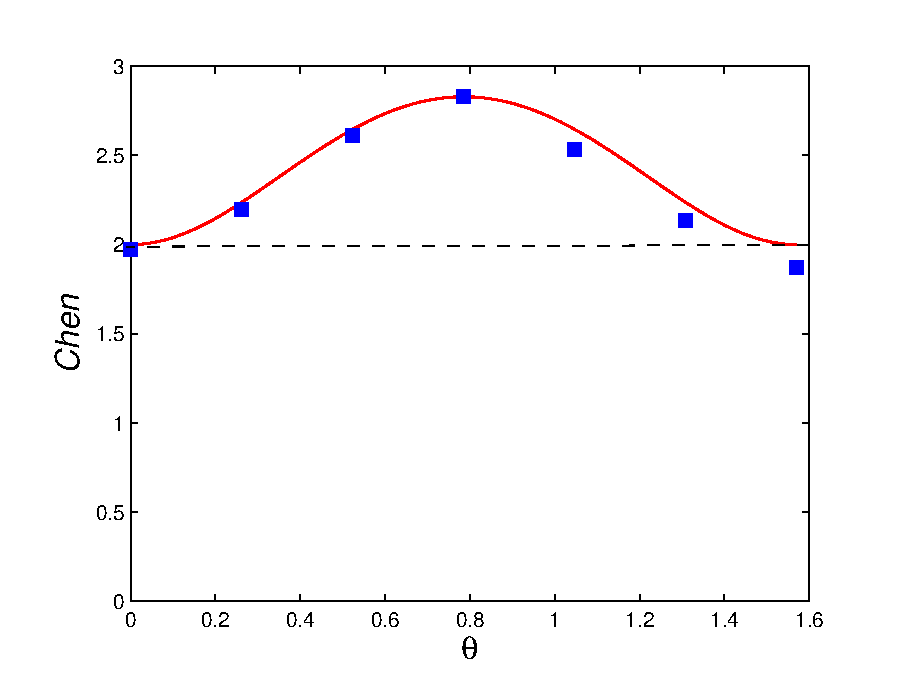
\includegraphics[width=0.35\textwidth]{Chen.eps}
\caption{\footnotesize{The values of $\mathcal{B}_{Chen}$ as a
function of $\theta$. The red thick line stands for the theoretical
result, and the blue square stands for the experiment result.}}
\end{figure}
The results are always larger than $2$ no matter whatever $\theta$
is. It illustrates that, the whole region of generalized GHZ states
can violate the inequality by a set of suitable observation angles.

Obviously, Chen's inequality is more efficient than MABK inequality
for generalized GHZ states. The experimental result is shown in
Fig.6, which perfectly simulates the violation of Chen's inequality
for generalize GHZ states. It shows that our experimental result
is in good agreement with quantum mechanical theory.

\end{frame}
\subsection*{V. Conclusions}
\begin{frame}
In summary, we have investigated the simulation of the violation of Bell-type inequalities, including MABK inequality and Chen's inequality for a three-qubit GHZ state as well as the generalized GHZ states in a NMR system. In the range of the generalized GHZ states, these experiments shows that Chen's inequality is more efficient than MABK inequality.  The experimental results are well in agreement with the expectation of quantum mechanics.

It is necessary to emphasize that, in strict, because NMR qubits are
many nuclear spins of atoms bounded together in a single molecule,
separated by a few angstroms, the NMR experiment is inherently
local. That is to say, our results are also consistent with the
classical theory,depending on whether we have considered the mixed
part $I_{2^n}$. Whereas, the meaning is that, when we experimentally
simulate the violation of different Bell-type inequalities for
arbitrary generalized three-qubit GHZ states in NMR, the results
excellently display the quantum predictions. It tells us, despite of
many existed disputes, NMR may contribute more on some fundamentals
of quantum mechanics. As a refined tool and technique for
experimentally realizing quantum computation in the last decade, NMR
is still contributing to numerous fundamental problems of quantum
mechanics now. In the future, we will still pay attention to this
area.
\end{frame}
\subsection*{Acknowledgments}
\begin{frame}
The authors are grateful to Ya Wang, Ping Zou and Jing Zhu for their
help and interesting comments and discussions. Financial support
comes from National Natural Science Foundation of China, the CAS,
Ministry of Education of PRC, and the National Fundamental Research
Program. It is also supported by Marie Curie Action program of the
European Union.
\end{frame}
\begin{thebibliography}{99}
\bibitem{Bell} J. S. Bell, Physics (Long Island city, N.Y) 1,195 (1964).
\bibitem{Stapp} H. P. Stapp, Nuovo Cimento Soc. Ital. Fis. B 29, 270 (1975).
\bibitem{Zukowski} M. \.{Z}ukowski, Stud. Hist. Phil. Mod. Phys. 36, 566 (2005).
\bibitem{CHSH} J. Clauser, M. Horne, A. Shimony, and R. Holt, Phys. Rev. Lett.
23, 880 (1969).
\bibitem{MABK} N. D. Mermin, Phys. Rev. Lett. 65, 1838 (1990); S. M. Roy and V. Singh, ibid. 67, 2761 (1991); M.
Ardehali, Phys. Rev. A 46, 5375 (1992); A. V. Belinskii and D. N.
Klyshko, Phys. Usp. 36, 653 (1993); N. Gisin and H.
Bechmann-Pasquinucci, Phys. Lett. A 246, 1 (1998).
\bibitem{WWZB} R. F. Werner and M. M. Wolf, Phys. Rev. A 64, 032112
(2001); M. \.{Z}ukowski and \v{C} Brukner, Phys. Rev. Lett. 88,
210401 (2002).
\bibitem{Brukner} \v{C} Brukner, M. \.{Z}ukowski, J. W Pan, and A. Zeilinger, Phys.
Rev. Lett. 92, 127901 (2004).
\bibitem{Brassard} G. Brassard, H. Buhrman, N. Linden, A. A. M��thot, A. Tapp, and F.
Unger, Phys. Rev. Lett. 96, 250401 (2006).
\bibitem{Scarani} V. Scarani, and N. Gisin, Phys. Rev. Lett. 87, 117901 (2001).
\bibitem{Chen} Z. B. Chen, Q. Zhang, X. H Bao, J. Schmiedmayer and J. W. Pan, Phys. Rev. A 73, 050302 (2006).
\bibitem{Acin and Gisin} A. Ac\'{i}n, N. Gisin, and L. Masanes, Phys. Rev. Lett. 97, 120405 (2006).
\bibitem{Barrett} J. Barrett, L. Hardy, and A. Kent, Phys. Rev. Lett. 95, 010503 (2005).
\bibitem{Acin and Brunner} A. Ac\'{i}n, N. Brunner, N. Gisin, S. Massar, S. Pironio, V. Scarani, Phys. Rev. Lett. 98, 230501 (2007).
\bibitem{Nielsen} M. A. Nielsen, and I. L. Chuang,  Quantum Computation and Quantum
Information (Cambridge: Cambridge University Press) (2000).
\bibitem{Freedman} S. J. Freedman and J. F. Clauser, Phys. Rev. Lett. 28, 938 (1972).
\bibitem{Aspect} A. Aspect, J. Dalibard, and G. Roger, Phys. Rev. Lett. 49, 1804 (1982).
\bibitem{Weihs} G. Weihs et al., Phys. Rev. Lett. 81, 5039 (1998).
\bibitem{Moehring} D. L. Moehring et al., Phys. Rev. Lett. 93, 090410 (2004).
\bibitem{Matsukevich1} D. N. Matsukevich et al., Phys. Rev. Lett. 95, 040405 (2005).
\bibitem{Matsukevich2} D. N. Matsukevich et al., Phys. Rev. Lett. 100, 150404 (2008).
\bibitem{Matsukevich3} D. N. Matsukevich et al., Phys. Rev. Lett. 96, 030405 (2006).
\bibitem{Chou} C.-W. Chou et al., Science 316, 1316 (2007).
\bibitem{Rowe} M. A. Rowe et al., Nature (London) 409, 791 (2001).
\bibitem{Souza} A. M. Souza et al., New. J. Phys. 10, 033020 (2008).
\bibitem{Lu} C. Y. Lu, (private communication).
\bibitem{Acin and Durt} A. Ac\'{i}n,, T. Durt, N. Gisin and J. I. Latorre, Phys. Rev. A 65, 052325 (2002).
\bibitem{Methot and Scarani} A.A. M\'{e}thot and V. Scarani, Quant. Inf. Comput. 7, 157 (2007).
\bibitem{k.Chen} K. Chen, S. Albeverio, and S. M. Fei, Phys. Rev. A 74, 050101(R)(2006).
\bibitem{Anwar} M. S. Anwar , D. Blazina \emph{et.al}, Phys. Rev. Lett. 93, 040501 (2004).
\bibitem{Scarani and Gisin} V. Scarani and N. Gisin, J. Phys. A 34, 6043 (2001).
\bibitem{Gershenfeld} N. A. Gershenfeld, I. L. Chuang, Science 275, 350-356
(1997).
\bibitem{Cory} D. G. Cory, A. F. Fahmy and T. F. Havel, Proc. Natl.
Acad, Sci. USA, 94:1634 (1997).
\bibitem{Fortunato} E. Fortunato \emph{et al.}, Chem. Phys. 116(17), 7599
(2002).
\bibitem{Zukowski and Brukner and Laskowski and Wiesniak} M. \.{Z}ukowski, \v{C} Brukner, W. Laskowski, and M. Wiesniak, Phys. Phys. Rev. Lett. 88, 210402 (2002).
\bibitem{J. L. Chen} J. L. Chen, C. F. Wu \emph{et al.}, Phys. Rev. Lett. 93, 140407 (2004).
\bibitem{C. F. Wu} C. F. Wu, J. L. Chen \emph{et al.}, Phys. Rev. A 77, 062309 (2008).

\end{thebibliography}

\end{document}
